\documentclass{article}

% Language setting
% Replace `english' with e.g. `spanish' to change the document language
\usepackage[english]{babel}
\usepackage{authblk}
\usepackage{amsthm, calc}
\usepackage{amsfonts}
\usepackage{graphicx}
\graphicspath{ {./images/} }
\newtheorem{definition}{Definition}
\newtheorem{theorem}{Theorem}


% Set page size and margins
% Replace `letterpaper' with `a4paper' for UK/EU standard size
\usepackage[letterpaper,top=2cm,bottom=2cm,left=3cm,right=3cm,marginparwidth=1.75cm]{geometry}

% Useful packages
\usepackage{amsmath}
\usepackage{graphicx}
\usepackage[colorlinks=true, allcolors=blue]{hyperref}

\title{Analysis of the Stability in Nonlinear Ordinary Differential Equations}
\author{Ranitha Mataraarachchi}
\affil{Department of Engineering Mathematics, Faculty of Engineering, University of Peradeniya, Peradeniya, Sri Lanka.}

\begin{document}
\maketitle

\section{Nonlinear Systems}
\subsection{Ordinary Differential Equations}

A differential equation is a mathematical equation involving one or more functions and their derivatives. The derivatives of these functions describe the rate of change of the functions at specific points. This mathematical concept finds widespread applications in various disciplines, including physics, engineering, biology, and more. The fundamental objective of differential equations is to investigate solutions (equilibrium points) of the specified equations and to analyze the characteristics of these solutions.

\begin{definition}
    An ordinary differential equation (ODE) is an equation which contains one or more terms and the derivatives of one variable with respect to the other variable. A \emph{n-th order} ordinary differential equation can be expressed as,
\begin{equation}
    x^{(n)}(t)=f(x^{(n-1)}(t),x^{(n-2)}(t),\dots,x'(t),x(t),t).
\end{equation}

where, $x^{(m)}=\frac{d^mx(t)}{dt^m}.$ The variable $t$ usually refers to the time in many practical systems.
\end{definition}

Most of the times it is convenient to represent this higher order differential equation as a system of first order differential equations. Therefore, we let $x_1=x(t), x_2=x_1'=x'(t), x_3=x_2'=x''(t),\dots,x_n=x_{n-1}'=x^{(n-1)}$, then $x_n'=x^{(n)} = f(x_1,x_2,\dots,x_n,t).$

From the above definition we get a system of first order differential equations that can be represented as,

\begin{align*}
  x_1' &= x_2\\
  x_2' &= x_3\\
     &\mathrel{\makebox[\widthof{=}]{\vdots}} \\
  x_{n-1}' &= x_n\\
  x_{n}' &= f(x_1,x_2,\dots,x_n,t).
\end{align*}

The above set of equations can be represented as,

\begin{align*}
  x_1' &= f_1(x_1,x_2,\dots,x_n,t)\\
  x_2' &= f_2(x_1,x_2,\dots,x_n,t)\\
     &\mathrel{\makebox[\widthof{=}]{\vdots}} \\
  x_{n}' &= f_n(x_1,x_2,\dots,x_n,t).
\end{align*}

Therefore, the system can be expressed in the vector notation as
\begin{equation}
    \dot{X} = F(X,t),
\end{equation}

where, $\dot{X}=[x_1',x_2',\dots,x_n']^T$, $X=[x_1,x_2,\dots,x_n]^T$ and $F=[f_1,f_2,\dots,f_n]^T$ are all $n$ dimensional vectors. Here we assume $F$ is a collection of continuous differentiable functions. From this, it is clear that any $n^{th}$ order ODE can be represented as a collection of (a system of) $n$ dimensional $1^{st}$ order ODEs.

\subsubsection{Autonomous Ordinary Differential Equations}

If the variable $t$ does not appear in the function $f$ explicitly, we refer to such equations as \emph{Autonomous ODEs}.

\begin{definition}
    A system of ordinary differential equations is called autonomous, if it has the form 
    \begin{equation}\label{auto}
        \dot{X} = F(X)
    \end{equation}
    
    for some vector valued function $F$.
\end{definition}

In this discussion we will limit our scope to Autonomous ODEs. 

\subsubsection{Linear Ordinary Differential Equations}

If all the elements belonging to $\dot{X}$ can be represented as a linear combination of the elements in $X$, then we call such a system a linear system. This is analogues to each $f_i \in F,i=1,2,\dots,n$ being a linear equation. 

\begin{definition}
    If for all $i=1,2,\dots,n$ there exists $a_{i1},a_{i2},\dots,a_{in} \in \mathbb{R}$ such that
    $$x_i' = \sum_{j=1}^n a_{ij} x_j,$$
    then we call this collection of ODEs a linear system. If the system is not linear, it is called a nonlinear system.
\end{definition}

Thus, the autonomous system in \eqref{auto} can be reduced to the matrix form

\begin{equation}\label{linear}
    \dot{X} = AX,
\end{equation}

where

\[
A = \begin{bmatrix}
    a_{11} & a_{12} & \hdots & a_{1n} \\
    a_{21} & a_{22} & \hdots & a_{2n} \\
    \vdots & \vdots & \ddots & \vdots \\
    a_{n1} & a_{n2} & \hdots & a_{nn} \\
\end{bmatrix}.
\]



\subsubsection{Equilibrium points of an Ordinary Differential Equation}

It is clear that for a system to achieve equilibrium the rate of change $\dot{X}$ must be $0$.
\begin{definition}
    An equilibrium of the n dimensional system $\dot{X} = F(X)$ is a vector $X^* \in \mathbb{R}^n$  such that $F(X^*)=0.$
\end{definition}


\section{Definition of Stability}
\subsection{Equilibrium point at the origin}
Consider the autonomous system $\dot{X} = F(X)$. Assume there exists an equilibrium point $X^*$, where $F(X^*)=0.$ Our objective is to analyze and define the stability of $X^*$. For convenience we state all definitions and theorems for the case when the equilibrium point is at the origin of $\mathbb{R}^n$; that is, $X^*=0.$ This choice is not restrictive, as any equilibrium point can be shifted to the origin through a variable transformation without loss of generality.

Suppose $X^*\neq0$ and consider the change of variables $Y=X-X^*$. This means we make $Y=[x_1-X^*,x_2-X^*,\dots,x_n-X^*]^T$. The derivative of $Y$ is given by 
$$\dot{Y}=\dot{X}=F(X)=F(Y+X^*)$$.
Now define
\begin{equation}
    G(Y) = F(Y+X^*)
\end{equation}
where $G(0)=0.$ By changing the variable we have shifted the equilibrium to the origin. Therefore, without loss of generality, we will assume $F(X)$ satisfies $F(0)=0$ and study the stability at the origin $0.$

\subsection{Stable, unstable and asymptotically stable systems}
\begin{definition}
    The equilibrium point $X=0$ of $\dot{X}=F(X)$ is
    \begin{itemize}
        \item \textbf{stable} if, for each $\epsilon > 0$, there is $\delta = \delta(\epsilon)>0$ such that
        $$\|X(0)\|<\delta \implies \|X(t)\|<\epsilon, \forall t\geq 0.$$

        \item \textbf{unstable} if it is not stable.

        \item \textbf{asymptotically stable} if it is stable \emph{and} $\delta$ can be chosen such that
        $$\|X(0)\|<\delta \implies \lim_{t \to \infty} X(t)=0.$$
    \end{itemize}
\end{definition}
Here, $\|\|$ represents the $L_2$ norm. The definition states that the system $F(X)$ with an equilibrium point at $X=0$ is \emph{stable} if for all the initial conditions within ball of (arbitrary) radius $\epsilon$ we can find a ball with some radius $\delta$ such that all the trajectories starting from within the ball of radius $\epsilon$ will always (i.e. $\forall t\geq 0$) stay within the ball of radius $\delta$. The system is said to be \emph{asymptotically stable} if it is stable and all the trajectories starting from within
the ball of radius $\epsilon$ will go to the origin (equilibrium point) as $t \to \infty.$ 

\section{Stability Analysis Using Linearization}
\subsection{Stability of linear systems}
Consider the linear system given in \eqref{linear}. This system has an equilibrium at the origin. We can determine the stability of such a system by observing the eigenvalues of $A.$ The solution of \eqref{linear} for a given initial state $X(0)$ is given by,
\begin{equation}\label{exp}
    X(t) = e^{At}X(0).
\end{equation}

For any matrix $A$ there is a non-singular matrix $P$ that transforms $A$ into its Jordan form. That is, 
$$P^{-1}AP = J = \text{ block diag }[J_1,J_2,\dots,J_r]$$
where $J_i$ is a Jordan block associated with the eigenvalue $\lambda_i$ of $A.$ Therefore,

\begin{equation}\label{sumsum}
    e^{At} = Pe^{Jt}P^{-1} = \sum_{i=1}^r\sum_{k=1}^{m_i}t^{k-1}e^{\lambda_i t}R_{ik}
\end{equation}


where $m_i$ is the order of the Jordan block $J_i$ and $R_{ik}$ is the matrix carrying all the residual terms. If an $n\times n$ matrix $A$ has a repeated eigenvalue $\lambda_i$ of algebraic multiplicity $q_i$, then the Jordan blocks associated with $\lambda_i$ have order one if and only if $rank(A-\lambda_i I) = n-q_i.$

\begin{theorem}\label{t1}
    The equilibrium point $X=0$ of $\dot{X}=AX$ is stable if and only if all eigenvalues $\lambda_i$ of $A$ satisfy $Re(\lambda_i)\leq0$ and for every eigenvalue with $Re(\lambda_i)=0$ and algebraic multiplicity $q_i\geq 2$, $rank(A-\lambda_i I)=n-q_i$, where $n$ is the dimension of $X$.  The equilibrium point $X=0$ is asymptotically stable if and only if all eigenvalues of $A$ satisfy $Re(\lambda_i)<0$.

\end{theorem}

\begin{proof}
    From \eqref{exp}, we can see that the origin is stable if and only if $e^{At}$ is a bounded function of $t$ for all $t\geq 0$. If one of the eigenvalues of $A$ is in the right-half complex plane the corresponding exponential term $e^{\lambda_i t}$ in \eqref{sumsum} will grow unbounded as $t\to \infty.$ Therefore, we must restrict the eigenvalues to be in the closed left-half complex plane. However, those eigenvalues in the imaginary axis $(Re(\lambda_i)=0)$, could give rise to unbounded terms if the order of an associated Jordan block is higher than one, due to the term $t^{k-1}$ in \eqref{sumsum} as $t\to\infty$. Therefore, we must restrict the eigenvalues on the imaginary axis to have Jordan block of order one, which is equivalent to the rank condition $rank(A-\lambda_i I) = n-q_i$. Thus we conclude the condition for stability is a necessary one. It is clear that the condition is also sufficient to ensure that $e^{At}$ is bounded. For asymptotic stability of the origin, $e^{At}$ must approach $0$ as $t\to\infty.$ From \eqref{sumsum}, this is the case if and only if $Re(\lambda_i)<0, \forall \lambda_i.$
\end{proof}

\subsection{Linearization of nonlinear systems at equilibrium points}
We can establish a theorem similar to theorem \eqref{t1} for nonlinear systems by linearizing the nonlinear system in the vicinity of equilibrium points. 

Let us first linearize the autonomous nonlinear system $\dot{X}=F(X)$ near the equilibrium point at the origin $(X=0).$ Since $F$ is a collection of continuous differentiable functions $[f_1,f_2,\dots,f_n]^T$, by the mean value theorem we can state

$$f_i(X) = f_i(0) + \left(\frac{\partial{f_i}}{\partial{x}}(Z_i)\right)X$$
for $i=1,2,\dots,n$ where $Z_i$ is a point on the line segment connecting $X$ to the origin and $\frac{\partial{f_i}}{\partial{x}} = [\frac{\partial{f_i}}{\partial{x_1}},\frac{\partial{f_i}}{\partial{x_2}},\dots,\frac{\partial{f_i}}{\partial{x_n}}]$. Since $F(0)=0$ we can write,

$$f_i(X) = \left(\frac{\partial{f_i}}{\partial{x}}(0)\right)X+\left[\left(\frac{\partial{f_i}}{\partial{x}}(Z_i)\right) - \left(\frac{\partial{f_i}}{\partial{x}}(0)\right)\right]X$$.
Hence,
\begin{equation}\label{approx}
    F(X) = AX + G(X)
\end{equation}
where

$$A = \left[\frac{\partial{f_1}}{\partial{x}}(0),\frac{\partial{f_2}}{\partial{x}}(0),\dots,\frac{\partial{f_n}}{\partial{x}}(0)\right]^T = \frac{\partial{f}}{\partial{x}}(0).$$
And 
$$G(X) = [g_1(X),g_2(X),\dots,g_n(X)]$$
where
$$g_i(X) = \left[\left(\frac{\partial{f_i}}{\partial{x}}(Z_i)\right) - \left(\frac{\partial{f_i}}{\partial{x}}(0)\right)\right]X.$$

for all $i=1,2,\dots,n.$

The function $g_i(X)$ satisfies

$$|g_i(X)| \leq \left\|\left(\frac{\partial{f_i}}{\partial{x}}(Z_i)\right) - \left(\frac{\partial{f_i}}{\partial{x}}(0)\right)\right\|\|X\|$$
where $\|\|$ represents the $L_2$ norm. By continuity of $\frac{\partial{f}}{\partial{x}}$, we see that
$$\left\|G(X)\right\|\to 0 \text{  as  } \|X\|\to 0.$$

This suggests that in a small neighbourhood of the origin \eqref{approx} reduces to $F(X) = AX$ and we can approximate the nonlinear system $\dot{X}=F(X)$ by its linearization about the origin 
$$\dot{X}=AX, \text{  where  } A=\frac{\partial{f}}{\partial{x}}(0).$$

\subsection{Stability of nonlinear systems by linearization}
The following theorem outlines conditions that allow us to make conclusions regarding the stability of the origin as an equilibrium point in a nonlinear system. This is achieved by examining its stability as an equilibrium point in the linear system. This theorem is referred to as \emph{Lyapunov's indirect method.}

\begin{theorem}\label{t2}
    Let $X=0$ be an equilibrium point for the nonlinear system
    $$\dot{X}=F(X)$$
    where all the functions $f_1,f_2,\dots,f_n$ in $F$ are continuously differentiable in the neighbourhood of the origin. Let 
    $$A=\frac{\partial{f}}{\partial{x}}(0).$$

    Then, 
    \begin{itemize}
        \item The origin is asymptotically stable if all eigenvalues $\lambda_i$ of $A$ satisfy $Re(\lambda_i)<0.$
        \item The origin is unstable if $Re(\lambda_i)>0$ for one or more eigenvalues of $A.$
    \end{itemize}
\end{theorem}
Here $A$ is the Jacobian matrix of $F$ evaluated at $X=0.$

\section{Lyapunov's Stability Theorem}
To determine the stability of a system we can use the concept of energy. If a system experiences a gradual reduction in energy over time during its motion trajectory, it will approach a stable equilibrium. Conversely, if the system undergoes an increase in energy over time during its trajectory, it may move away from a stable equilibrium. If there is neither a loss nor gain of energy, the system will persist in its current trajectory. Therefore, it is desirable to investigate the variation of energy of a system with respect to time as the system evolves. This concept is the essence of Lyapunov's stability theory. 

\begin{theorem}\label{t3}
    Let $X=0$ be an equilibrium point for the system $\dot{X}=F(X)$ and $D \subset \mathbb{R}^n$ be a domain containing $X=0.$ Let $V:D\to \mathbb{R}$ be a continuously differentiable function such that 
    $$V(0)=0 \text{  and  } V(X)>0 \text{  for  } X\in D\setminus \{0\}.$$
    If 
    $$\frac{dV(X)}{dt}\leq 0 \text{  for  } X\in D,$$
    then $X=0$ is stable. Moreover, if
    $$\frac{dV(X)}{dt} < 0 \text{  for  } X\in  D\setminus \{0\}$$
    then $X=0$ is asymptotically stable.
\end{theorem}

Here $V(X)$ is referred to as the \emph{Lyapunov's function} and it can be regarded as a measure of energy of the system.

\textbf{Example 1:} Consider the autonomous nonlinear system

\begin{align*}
  \dot{x_1} &= -x_1^3-x_2\\
  \dot{x_2} &= x_1 - x_2^3.
\end{align*}
The origin is an equilibrium point for this system. We will consider the function 
$$V(X) = \frac{x_1^2}{2}+\frac{x_2^2}{2}$$
Clearly $V(X)>0, \forall x_1,x_2.$ Then, by the chain rule of differentiation, 
$$\frac{dV(X)}{dt} = \frac{\partial{V(X)}}{\partial{x}}\frac{dX}{dt} = -(x_1^4+x_2^4).$$
Therefore, we have $\frac{dV}{dt}=-(x_1^4+x_2^4)<0$ whenever $X=(x_1,x_2)\neq (0,0) = 0.$ Thus, by theorem \eqref{t3} we can conclude that the above system is \emph{asymptotically stable} at the equilibrium point $X=0.$

\section{Lotka-Volterra Predator vs. Prey Model}
The Lotka–Volterra predator–prey model comprises a set of two first-order nonlinear differential equations commonly used to depict the dynamics of biological systems involving two interacting species, one acting as a predator and the other as prey. The evolution of populations over time is governed by the following pair of equations:
\begin{align*}
  \dot{x_1} &= ax_1-bx_1x_2\\
  \dot{x_2} &= -cx_2 + dx_1x_2.
\end{align*}
Here $x_1,x_2$ are the population densities of pray and predators respectively. $\dot{x_1},\dot{x_2}$ are the instantaneous growth rates of the two populations and $t$ represents time. $a$ and $b$ represent, respectively, the highest per capita growth rate of prey and the impact of predator presence on the rate of prey growth. $c$ and $d$, respectively, characterize the per capita death rate of predators and the influence of prey presence on the predator's growth rate. All parameters $a,b,c,d$ are positive and real.

We can represent this system as
\begin{equation}\label{lotka}
    \dot{X}=F(X).
\end{equation}

The system in \eqref{lotka} has two equilibrium points: $(0,0)$ (trivial equilibrium point) and $(\frac{c}{d},\frac{a}{b})$ (nontrivial equilibrium point). It is worthwhile to analyse both of these points individually. 

\subsection{ Trivial equilibrium point}

We can linearize the system in a neighbourhood of the equilibrium point to analyse the stability. We will find the eigenvalues of the matrix $A = \frac{\partial{f}}{\partial{x}}(0)$ to discuss the stability. Here $f_1(x_1,x_2)=ax_1-bx_1x_2$ and $f_2(x_1,x_2) = -cx_2 - dx_1x_2.$
We get
\[
A = \begin{bmatrix}
    \frac{\partial{f_1}}{\partial{x_1}} & \frac{\partial{f_1}}{\partial{x_2}} \\\\
    \frac{\partial{f_2}}{\partial{x_1}} & \frac{\partial{f_2}}{\partial{x_2}}
\end{bmatrix} = \begin{bmatrix}
    a & -bx_1 \\
    -dx_2 & -c
\end{bmatrix}.
\]
Upon evaluating the above matrix at the equilibrium point $(0,0)$ we get 

\[
A =  \begin{bmatrix}
    a & 0 \\
    0 & -c
\end{bmatrix}.
\]
Since the eigenvalues of a diagonal matrix are equal to its diagonal entries we see that the eigenvalues are $\lambda_1=a$ and $\lambda_2=-c.$ Notice that the parameters $a,b,c,d$ are always positive. Therefore, we get a positive eigenvalue for the above matrix. Thus by theorem \eqref{t2} we conclude that the equilibrium point $(0,0)$ is unstable. 

\subsection{Nontrivial equilibrium point}
We will try to linearize the system \eqref{lotka} and analyse the stability. Since the equilibrium point is not at the origin, we need to change the variables to achieve a system that has the equilibrium point at the origin. We will change the variables $(x_1,x_2)$ to $(y_1,y_2)$ by the relationship
\begin{align*}
  y_1 &= x_1-\frac{c}{d}\\
  y_2 &= x_2 - \frac{a}{b}.
\end{align*}
Therefore, the system can be rewritten as 
\begin{align*}
  \dot{y_1} &= -by_1y_2-\frac{bcy_2}{d}\\
  \dot{y_2} &= dy_1y_2+\frac{ady_1}{b}.
\end{align*}
by changing the variables. This new system 
\begin{equation}\label{new}
    \dot{Y} = G(Y)
\end{equation}
has an equilibrium point at $(0,0)$. Now, we will find the eigenvalues of the matrix $A = \frac{\partial{g}}{\partial{y}}(0)$ to discuss the stability. Here $g_1(y_1,y_2)=-by_1y_2-\frac{bcy_2}{d}$ and $g_2(y_1,y_2) = -dy_1y_2+\frac{ady_1}{b}.$ We get 
\[
A = \begin{bmatrix}
    \frac{\partial{g_1}}{\partial{y_1}} & \frac{\partial{g_1}}{\partial{y_2}} \\\\
    \frac{\partial{g_2}}{\partial{y_1}} & \frac{\partial{g_2}}{\partial{y_2}}
\end{bmatrix} = \begin{bmatrix}
    -by_2 & -\frac{bc}{d}-by_1 \\
    -dy_2 +\frac{ad}{b}& -dy_1
\end{bmatrix}.
\]
Upon evaluating the above matrix at the equilibrium point $(0,0)$ we get 

\[
A =  \begin{bmatrix}
    0 & -\frac{bc}{d} \\
    \frac{ad}{b} & 0
\end{bmatrix}.
\]

The eigenvalues of the above matrix are $\lambda_1=i\sqrt{ac}$ and $\lambda_2=-i\sqrt{ac}.$ Stability analysis by linearization is inconclusive at this equilibrium point since the eigenvalues for the linearized system at this point are purely imaginary. 

Therefore, we resolve to conduct stability analysis using the Lyapunov's method. We will investigate the nonlinear system $\dot{Y}=G(Y)$ developed above. This system has an equilibrium point at $(0,0)$. Consider the function 
\begin{equation}\label{energy}
    V(y_1,y_2) = dy_1 - c \ln\left(\frac{dy_1+c}{d}\right)+by_2- a \ln\left(\frac{by_2+a}{b}\right)+K,
\end{equation}

where $a,b,c,d$ are the parameters in \eqref{lotka} and $K$ is a constant. Then, by differentiating we see that
$$\frac{V(Y)}{dt}=0.$$ Thus, by theorem \eqref{t3} we can conclude that the above system is \emph{stable} at the equilibrium point $Y=(0,0)$ which corresponds with the equilibrium point $X=(\frac{c}{d},\frac{a}{b})$ in the system \eqref{lotka}.

\subsection{Numerical Simulation}
We will simulate the Lotka-Volterra predator vs prey model described in \eqref{lotka}. Let the parameters be equal to,

\begin{align*}
  a &= 0.1\\
  b &= 0.02 \\
  c &= 0.1 \\
  d &= 0.01.
\end{align*}

Clearly, $(0,0)$ is the trivial equilibrium point and $(10,5)$ is a nontrivial equilibrium point. We will first plot the vector $f_1(x_1,x_2)i+f_2(x_1,x_2)j$ at some selected initial values $(x_1,x_2)$. Here $i$ and $j$ are the unit vectors along the $x_1$ axis (horizontal) and $x_2$
axis (vertical) respectively. This gives a good graphical representation of the “flow” direction of the solution trajectories on the phase plane.

\begin{figure}[h]
\centering
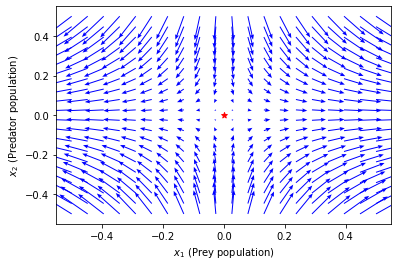
\includegraphics[scale=0.75]{images/origin.png}
\caption{Flow lines near the equilibrium point at the origin.}
\label{origin}
\end{figure}

\begin{figure}[h]
\centering
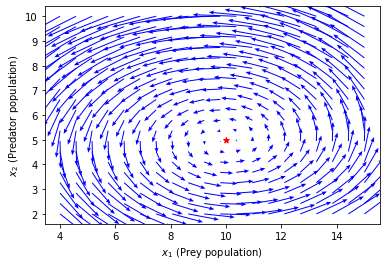
\includegraphics[scale=0.75]{images/nontrivial.png}
\caption{Flow lines near the nontrivial equilibrium point.}
\label{nontr}
\end{figure}

The figures \ref{origin} and \ref{nontr} indicates the flow direction of the solution trajectories near the equilibrium points $(0,0)$ and $(10,5)$ respectively. We can observe that the trivial equilibrium point is \emph{unstable} (in fact it is a saddle point) and the nontrivial equilibrium point attracts the solution trajectories to a cycle around it. 

By solving the system numerically with a time step $(\Delta t)$ of $0.01$ for $64$ initial values we get solution trajectories as seen in figure \ref{traj}. We solve only for non-zero initial conditions since zero initial conditions exhibit unstable behaviour. 

\begin{figure}[h]
\centering
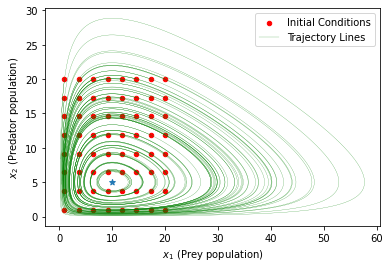
\includegraphics[scale=0.75]{images/init.png}
\caption{Solution trajectories for non-zero initial conditions.}
\label{traj}
\end{figure}

From the figure \ref{traj} we can observe that the solution trajectories tend to revolve around cycles centered around the nontrivial equilibrium point. It is visible that for non-zero initial conditions the population levels of predators and preys can arbitrary drop towards extinction but can recover and revolve around a cycle around the nontrivial equilibrium point. 

We can solve \eqref{lotka} analytically to get
$$W(x_1,x_2) = ax_1+b\ln{x_1}-cx_2+d\ln{x_2}+K$$
where $K$ is an arbitrary constant. This describes the population dynamics of the population. We can plot $W(X)$ by setting $K=10$. Figure \ref{W} shows this variation. We can observe that the nontrivial equilibrium point $(10,5)$ acts as a minima of this function. 

\begin{figure}[h]
\centering
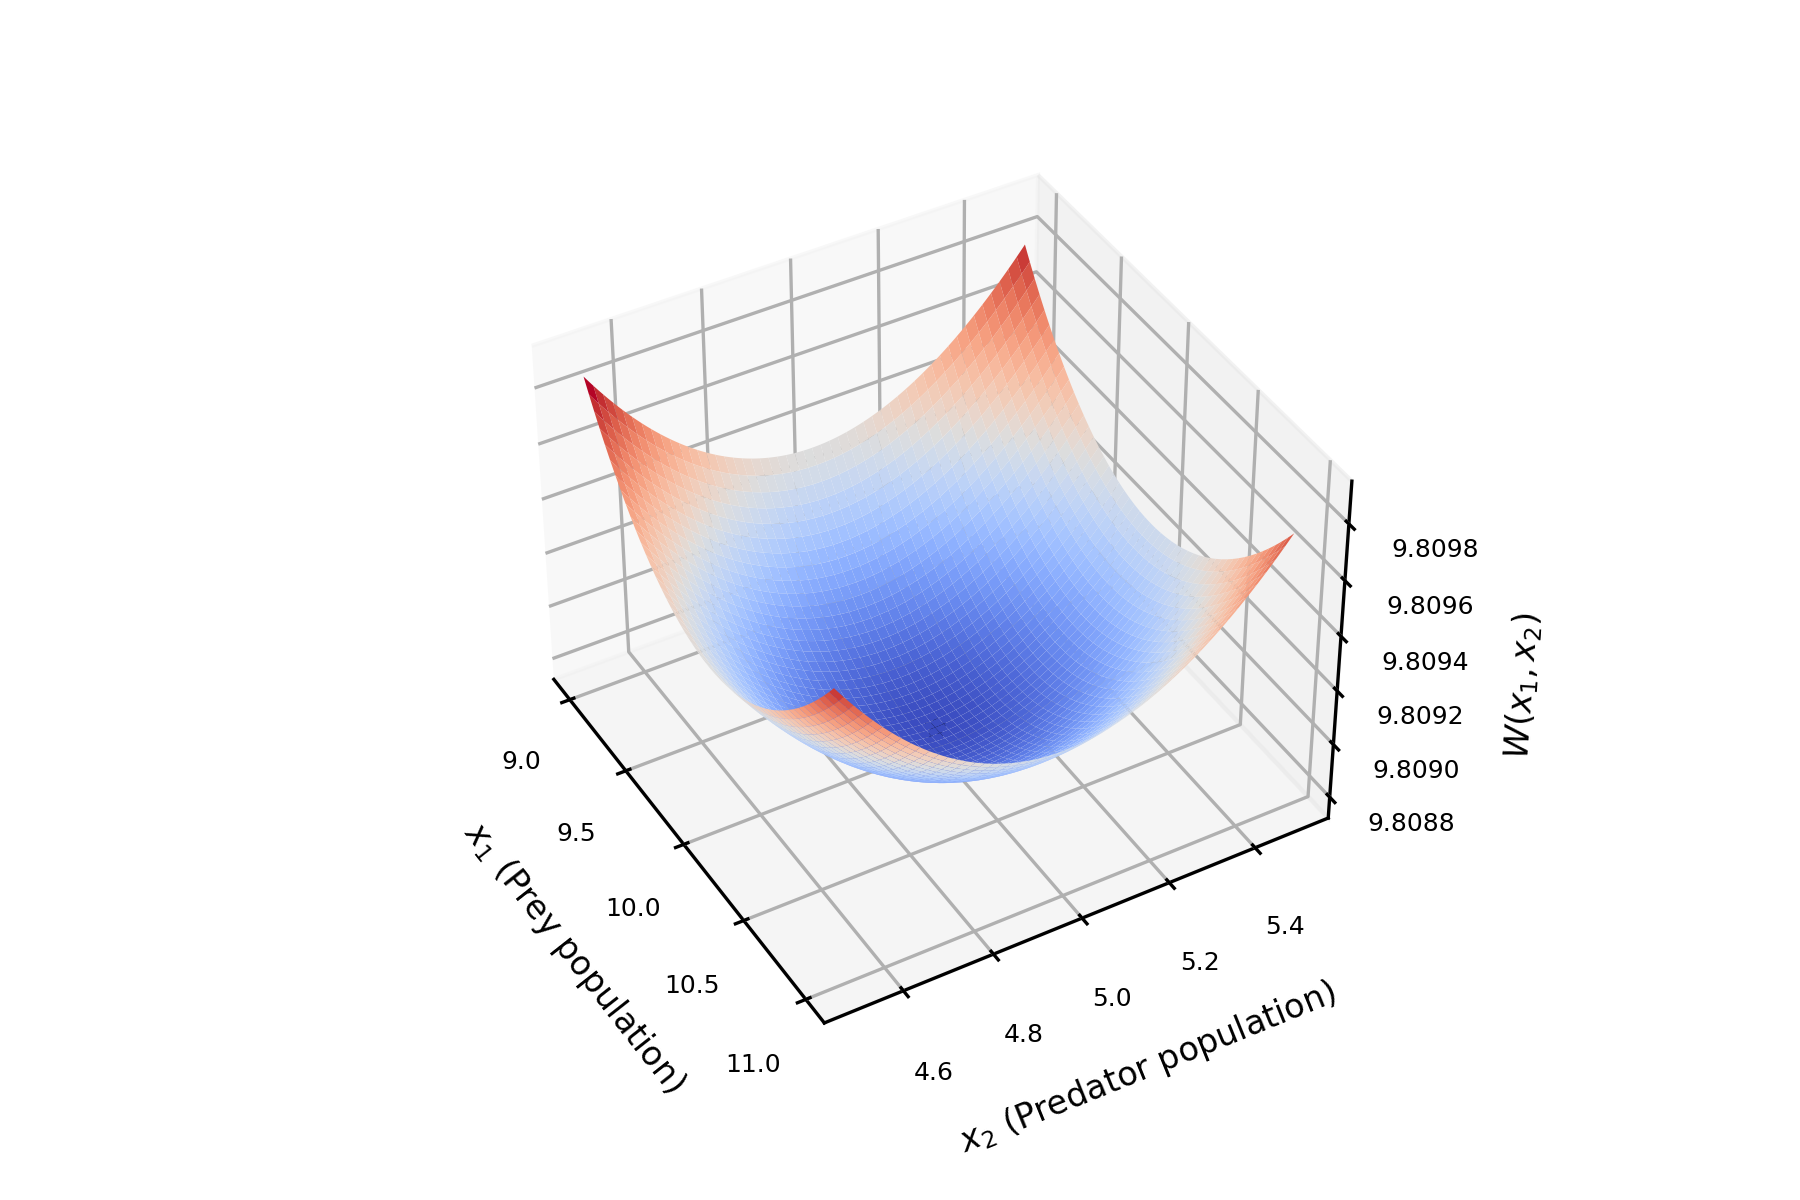
\includegraphics[scale=0.75]{images/larger_plot.png}
\caption{Variation of $W(X)$ with $x_1$ and $x_2$.}
\label{W}
\end{figure}

\nocite{*}
\bibliographystyle{plain}
\bibliography{sample}

\end{document}